\documentclass{article}

\usepackage{fancyhdr}
\usepackage{extramarks}
\usepackage{amsmath}
\usepackage{amsthm}
\usepackage{amsfonts}
\usepackage{tikz}
\usepackage[plain]{algorithm}
\usepackage{algpseudocode}
\usepackage{enumerate}
\usepackage{tikz}

\usetikzlibrary{automata,positioning}

%
% Basic Document Settings
%  

\topmargin=-0.45in
\evensidemargin=0in
\oddsidemargin=0in
\textwidth=6.5in
\textheight=9.0in
\headsep=0.25in

\linespread{1.1}

\pagestyle{fancy}
\lhead{\hmwkAuthorName}
\chead{\hmwkClass : \hmwkTitle}
\rhead{\firstxmark}
\lfoot{\lastxmark}
\cfoot{\thepage}

\renewcommand\headrulewidth{0.4pt}
\renewcommand\footrulewidth{0.4pt}

\setlength\parindent{0pt}

%
% Create Problem Sections
%

\newcommand{\enterProblemHeader}[1]{
    \nobreak\extramarks{}{Problem \arabic{#1} continued on next page\ldots}\nobreak{}
    \nobreak\extramarks{Problem \arabic{#1} (continued)}{Problem \arabic{#1} continued on next page\ldots}\nobreak{}
}

\newcommand{\exitProblemHeader}[1]{
    \nobreak\extramarks{Problem \arabic{#1} (continued)}{Problem \arabic{#1} continued on next page\ldots}\nobreak{}
    \stepcounter{#1}
    \nobreak\extramarks{Problem \arabic{#1}}{}\nobreak{}
}

\newcommand*\circled[1]{\tikz[baseline=(char.base)]{
		\node[shape=circle,draw,inner sep=2pt] (char) {#1};}}


\setcounter{secnumdepth}{0}
\newcounter{partCounter}
\newcounter{homeworkProblemCounter}
\setcounter{homeworkProblemCounter}{1}
\nobreak\extramarks{Problem \arabic{homeworkProblemCounter}}{}\nobreak{}

%
% Homework Problem Environment
%
% This environment takes an optional argument. When given, it will adjust the
% problem counter. This is useful for when the problems given for your
% assignment aren't sequential. See the last 3 problems of this template for an
% example.
%

\newenvironment{homeworkProblem}[1][-1]{
    \ifnum#1>0
        \setcounter{homeworkProblemCounter}{#1}
    \fi
    \section{Problem \arabic{homeworkProblemCounter}}
    \setcounter{partCounter}{1}
    \enterProblemHeader{homeworkProblemCounter}
}{
    \exitProblemHeader{homeworkProblemCounter}
}

%
% Homework Details
%   - Title
%   - Class
%   - Due date
%   - Name
%   - Student ID

\newcommand{\hmwkTitle}{Homework\ \#12}
\newcommand{\hmwkClass}{Probability \& Statistics for EECS}
\newcommand{\hmwkDueDate}{May 7, 2023}
\newcommand{\hmwkAuthorName}{Zhou Shouchen}
\newcommand{\hmwkAuthorID}{2021533042}


%
% Title Page
%

\title{
    \vspace{2in}
    \textmd{\textbf{\hmwkClass:\\  \hmwkTitle}}\\
    \normalsize\vspace{0.1in}\small{Due\ on\ \hmwkDueDate\ at 23:59}\\
	\vspace{4in}
}

\author{
	Name: \textbf{\hmwkAuthorName} \\
	Student ID: \hmwkAuthorID}
\date{}

\renewcommand{\part}[1]{\textbf{\large Part \Alph{partCounter}}\stepcounter{partCounter}\\}

%
% Various Helper Commands
%

% Useful for algorithms
\newcommand{\alg}[1]{\textsc{\bfseries \footnotesize #1}}
% For derivatives
\newcommand{\deriv}[1]{\frac{\mathrm{d}}{\mathrm{d}x} (#1)}
% For partial derivatives
\newcommand{\pderiv}[2]{\frac{\partial}{\partial #1} (#2)}
% Integral dx
\newcommand{\dx}{\mathrm{d}x}
% Alias for the Solution section header
\newcommand{\solution}{\textbf{\large Solution}}
% Probability commands: Expectation, Variance, Covariance, Bias
\newcommand{\E}{\mathrm{E}}
\newcommand{\Var}{\mathrm{Var}}
\newcommand{\Cov}{\mathrm{Cov}}
\newcommand{\Bias}{\mathrm{Bias}}

\begin{document}

\maketitle

\pagebreak

\begin{homeworkProblem}[1]
(a) Since the prior distribution of $p$ is $Unif(0,1)$, which is exactly same as $Beta(1,1)$.\\
This is because $\beta(1,1)=\int_{0}^{1}x^{1-1}(1-x)^{1-1}dx=1,x\in(0,1)$, then $\dfrac{1}{\beta(1,1)}x^{1-1}(1-x)^{1-1}=1,x\in(0,1)$.\\
So the prior distribution is that $p\sim Beta(1,1)$.\\
From what we have learned about the Bayesian Inference,\\
we can calculate the posterior distribution of $p$:\\
Since $X_i|p\sim Bern(p)$, so $S = \sum\limits_{i=1}^n X_i|p\sim Bin(n,p)$,\\
with Beta-Binomial conjugate prior, we can get the posterior is that:\\
$(p|X_1=x_1,\cdots,X_n=x_n)=(p|S=k)\sim Beta(1+\sum\limits_{i=1}^n x_i,1+n-\sum\limits_{i=1}^n x_i)$.\\

So above all, the posterior distribution of $p$ given $X_1=x_1,\cdots,X_n=x_n$ is that:\\
$p|X_1=x_1,\cdots,X_n=x_n\sim Beta(1+\sum\limits_{i=1}^n x_i,1+n-\sum\limits_{i=1}^n x_i)$.\\
And we can see that it only depends on the sum of $x_i$.\\

(b) With LOTP, we can get that\\
$$P(X_{n+1}=1|X_1+\cdots+X_n=k)=\int_{0}^{1}P(X_{n+1}=1|X_1+\cdots+X_n=k,p=p')f_p(p'|X_1+\cdots+X_n=k)dp'$$
From (a), we know that $p|X_1=x_1,\cdots,X_n=x_n\sim Beta(1+k,1+n-k)$,\\
so $f_p(p'|X_1+\cdots+X_n=k)=\dfrac{1}{\beta(1+k,1+n-k)}p'^{1+k-1}(1-p')^{1+n-k-1}=\dfrac{1}{\beta(1+k,1+n-k)}p'^{k}(1-p')^{n-k}$.\\
So the above equation can be written as:\\
$$=\int_{0}^{1}P(X_{n+1}=1|X_1+\cdots+X_n=k,p=p')\dfrac{1}{\beta(1+k,1+n-k)}p'^{k}(1-p')^{n-k}dp'$$
And since $X_i|p$ are conditional independent $Bin(p)$,\\
so $P(X_{n+1}=1|X_1+\cdots+X_n=k,p=p')=P(X_{n+1}=1|p=p')=p'$,\\
So the above equation can be written as:\\
$$=\dfrac{1}{\beta(1+k,1+n-k)}\int_{0}^{1}p'p'^{k}(1-p')^{n-k}dp'$$
Since $\beta(a,b)=\dfrac{\Gamma(a)\Gamma(b)}{\Gamma(a+b)}$, and when $a,b$ are positive integers, $\Gamma(a)=(a-1)!$, so $\beta(a,b)=\dfrac{(a-1)!(b-1)!}{(a+b-1)!}$.\\
From the problem's description, we can get that both $1+k$ and $1+n-k$ are positive integers, so $\beta(1+k,1+n-k)=\dfrac{k!(n-k)!}{(n+1)!}$.\\
Also, we can see that $\int_{0}^{1}p'p'^{k}(1-p')^{n-k}dp'=\int_{0}^{1}p'^{k+1}(1-p')^{n-k}dp'=\beta(k+2,n-k+1)$.\\
From above analysis, we can also get that k+2,n-k+1 are positive integers.\\
So $\beta(k+2,n-k+1)=\dfrac{\Gamma(k+2)\Gamma(n-k+1)}{\Gamma(k+2+n-k+1)}=\dfrac{(k+1)!(n-k)!}{(n+2)!}$.\\
So the above equation can be written as:\\
$$=\dfrac{1}{\dfrac{k!(n-k)!}{(n+1)!}}\dfrac{(k+1)!(n-k)!}{(n+2)!}=\dfrac{k+1}{n+2}$$

So above all, $P(X_{n+1}=1|X_1+\cdots+X_n=k)=\dfrac{k+1}{n+2}$.\\

(c) Reinterpret the Laplaces's law of succession from the persoective of Beta-Binomial conjugacy is that:\\
From the view of Bayesian Inference, we get a prior distribution of $p$ is that $p\sim Unif(0,1)\sim Beta(1,1)$.\\
And the $n$ variables $X_1,\cdots,X_n$ are conditional independent $Bern(p)$, i.e. $X_i|p\sim Bern(p)$.\\
From this we can get that $\sum\limits_{i=1}^nX_i|p=X$, $X\sim Bin(n,p)$.\\
And from the Beta-Binomial conjugacy we can get the posterior distribution of $p$ given $X_1=x_1,\cdots,X_n=x_n$ is that:\\    
$p|X_1=x_1,\cdots,X_n=x_n\sim Beta(1+\sum\limits_{i=1}^n x_i,1+n-\sum\limits_{i=1}^n x_i)$.\\
And we can see that it only depends on the sum of $x_i$.\\
So with the posterior distribution $p|X_1=x_1,\cdots,X_n=x_n$, we can calculate the newly inference:\\
$P(X_{n+1}=1|X_1+\cdots+X_n=k)=\dfrac{k+1}{n+2}$.\\

So above all is the perspective of Beta-Binomial Conjugacy to see the Laplaces's law of succession.\\

\end{homeworkProblem}

\newpage

\begin{homeworkProblem}[2]
(a) Since $p\sim Beta(a,b)$, so from LOUTS, we can get that\\
$E[p^2(1-p)^2]=\int_{0}^{1}\dfrac{1}{\beta(a,b)}p^{a-1}(1-p)^{b-1}\cdot p^2(1-p)^2dp=\dfrac{1}{\beta(a,b)}\int_{0}^{1}p^{a+1}(1-p)^{b+1}dp$.\\
And since $\int_{0}^{1}p^{a+1}(1-p)^{b+1}dp=\beta(a+2,b+2)$.\\
So $E[p^2(1-p)^2]=\dfrac{\beta(a+2,b+2)}{\beta(a,b)}$.\\
Since $a,b$ are positive real numbers, so $\beta(a,b)=\dfrac{\Gamma(a)\Gamma(b)}{\Gamma(a+b)}$, similarly, $\beta(a+2,b+2)=\dfrac{\Gamma(a+2)\Gamma(b+2)}{\Gamma(a+b+4)}$.\\
Also, since $a,b$ are positive real numbers, so $\Gamma(a+2)=(a+1)\Gamma(a+1)=(a+1)a\Gamma(a)$, similarly, $\Gamma(b+2)=(b+1)\Gamma(b+1)=(b+1)b\Gamma(b)$.\\
So $\beta(a+2,b+2)=\dfrac{(a+1)a\Gamma(a)(b+1)b\Gamma(b)}{(a+b+3)(a+b+2)(a+b+1)(a+b)\Gamma(a+b)}$.\\
So $E[p^2(1-p)^2]=\dfrac{\beta(a+2,b+2)}{\beta(a,b)}=\dfrac{\Gamma(a+b)}{\Gamma(a)\Gamma(b)}\cdot\dfrac{(a+1)a\Gamma(a)(b+1)b\Gamma(b)}{(a+b+3)(a+b+2)(a+b+1)(a+b)\Gamma(a+b)}$.\\
$=\dfrac{(a+1)a(b+1)b}{(a+b+3)(a+b+2)(a+b+1)(a+b)}$.\\

So above all, $E[p^2(1-p)^2]=\dfrac{(a+1)a(b+1)b}{(a+b+3)(a+b+2)(a+b+1)(a+b)}$.\\

(b) It only depends on the fact that $A$ won exactly $6$ of the $10$ games on record.\\

According to what we have learn about Bayesian Inference, we can get that:\\
The prior distribution of $p$ is $Unif(0,1)$.\\
And since $\beta(1,1)=\dfrac{\Gamma(1)\Gamma(1)}{\Gamma(2)}=1$, so $Unif(0,1)\sim Beta(1,1)$,
i.e.the prior distribution of $p\sim Beta(1,1)$.\\

And for the historical data, the winners are $AAABBABAB$.\\
Let $X_i$ records the i-th pervious data, if $A$ won the game, then $X_i=1$, otherwise $X_i=0$.\\
So $X_1=1,X_2=1,X_3=1,X_4=0,X_5=0,X_6=1,X_7=1,X_8=0,X_9=1,X_{10}=0$.\\

And we can get that $X_i|p\sim Bern(p)$, so $S=\sum\limits_{i=1}^{10}X_i|p\sim Bin(10,p)$. And $S=6$.\\
According to the Beta-Binomial conjugacy, we can get that the posterior distribution of $p$ only depends on the sum of $X_i$ i.e. $S$.\\ 
And we can get that $S=6$, for the total historical data of $10$ games, $A$ won $6$ games.\\

So according to the Beta-Binomial conjugacy, since the prior distribution $p\sim Beta(1,1)$,\\
so we can get that the posterior distribution of $p$ given $S=6$ is that:\\
$p|S=6\sim Beta(1+6,1+(10-6))\sim Beta(7,5)$.\\
i.e. $p|historical\ data\sim Beta(7,5)$.\\

So above all, the posterior distribution of $p$ only depends on the number of wins for $A$ in the $10$ games on record.\\

(c) From the analysis in (b), we can get that the prior distribution $p\sim Beta(0,1)$,\\
and $S=\sum\limits_{i=1}^{10}X_i|p\sim Bin(10,p)$, so the posterior distribution of $p$ given $S=6$ is that:\\
$p|historical\ data\sim Beta(1+6,1+(10-6))\sim Beta(7,5)$.\\ 

So above all, the posterior distribution of $p$ given the historical data is that $p|historical\ data\sim Beta(7,5)$.\\

(d) 1. Conditioning on $p$, the indicator of $A$ winning in the first game of the match $\textbf{uncorrelated with}$ the indicator of $A$ winning in the second game of the match.\\

According to the analysis in (b),(c), and according to what we have learned about Bayesian Inference, with given $p$, the first game and the second game are conditionally independent.\\

So they are uncorrelated.\\

2. Conditioning on the historical data, the indicator of $A$ winning in the first game of the match\\
$\textbf{positively correlated with}$ the indicator of $A$ winning in the second game of the match.\\

Without given $p$, we can intuitive regard that winning in the first game of the match could increases the estimation of $p$, it can also increase the belief that $A$ will win the next i.e. second game, and vise versa.\\
So winning the first game increases the probability of winning the second game that we are estmating, and vise versa.\\

So they are positively correlated.\\

(e) Since the match is not yet decided when going into the fifth games, the the first four games must tied, i.e. $A$ wins 2 games, and $B$ wins 2 games.\\
With the given historical data, i.e. with given $p$, we can get that $A$ has the probability of $p$ to win each game.\\
So for the situation that $A$ only wins 2 games in the first four games, the probability that this situation happens is that ${4\choose 2}p^2(1-p)^2$.\\

And from (c), we have known that $p\sim Beta(7,5)$, and from (a), we get that when $p\sim Beta(a,b)$, $E[p^2(1-p)^2]=\dfrac{(a+1)a(b+1)b}{(a+b+3)(a+b+2)(a+b+1)(a+b)}$.\\

So we can get the expectation of ${4\choose 2}p^2(1-p)^2$ is that:\\
$E[{4\choose 2}p^2(1-p)^2]={4\choose 2}E[p^2(1-p)^2]$\\
$={4\choose 2}\dfrac{(a+1)a(b+1)b}{(a+b+3)(a+b+2)(a+b+1)(a+b)}={4\choose 2}\dfrac{8*7*6*5}{15*14*13*12}=\dfrac{4}{13}$\\

So above all, given the historical data, the expected value for the probability that the match is not yet decided when going into the fifth games is that $\dfrac{4}{13}$.\\

\end{homeworkProblem}

\newpage

\begin{homeworkProblem}[3]
(a) Since $U_1,\cdots,U_n\sim Unif(0,1)$, so $f(x)=1, 0<x<1$. And $F(x)=x,0<x<1$\\
The joint PDF of $U_{(1)},\cdots,U_{(n)}$ is $f_{U_{(1)},\cdots,U_{(n)}}(u_1,\cdots,u_n)=\lim\limits_{\delta_1,\cdots,\delta_n\to 0}\dfrac{P(U_{(1)}\in(u_1-\delta,u_1+\delta),\cdots,U_{(n)}\in(u_n-\delta,u_n+\delta))}{(2\delta_1)\cdots(2\delta_n)}$.\\
For $U_1,\cdots,U_n$, there are total $n!$ permutations, and for each permutation, suppose that $U_i$ be the i-th order statistic, so we can get that:\\
$\lim\limits_{\delta_1,\cdots,\delta_n\to 0}\dfrac{P(U_1\in (u_1-\delta_1,u_1+\delta_1),\cdots,U_n\in(u_n-\delta_n,u_n+\delta_n))}{(2\delta_1)\cdots(2\delta_n)}$\\
$=f(u_1)\cdots f(u_n)=1$.\\

So $\lim\limits_{\delta_1,\cdots,\delta_n\to 0}\dfrac{P(U_{(1)}\in(u_1-\delta,u_1+\delta),\cdots,U_{(n)}\in(u_n-\delta,u_n+\delta))}{(2\delta_1)\cdots(2\delta_n)}$\\
$=n!\cdot \lim\limits_{\delta_1,\cdots,\delta_n\to 0}\dfrac{P(U_1\in (u_1-\delta_1,u_1+\delta_1),\cdots,U_n\in(u_n-\delta_n,u_n+\delta_n))}{(2\delta_1)\cdots(2\delta_n)}=n!$.\\
i.e. $f_{U_{(1)},\cdots,U_{(n)}}(u_1,\cdots,u_n)=n!,u_1\leq u_2\leq\cdots u_n$.\\
And otherwise, $f_{U_{(1)},\cdots,U_{(n)}}(u_1,\cdots,u_n)=0$.\\

So above all, the joint PDF of $U_{(1)},\cdots,U_{(n)}$ is that\\
$f_{U_{(1)},\cdots,U_{(n)}}(u_1,\cdots,u_n)=n!,u_1\leq u_2\leq\cdots u_n$\\
$f_{U_{(1)},\cdots,U_{(n)}}(u_1,\cdots,u_n)=0, otherwise$.\\

(b) For the joint PDF of $U_{(j)}$ and $U_{(k)}$, since $1\leq j<k\leq n$,
considering that they are in a small interval $U_{(j)}\in(u_j-\delta_1,u_j+\delta_1)$, $U_{(k)}\in(u_k-\delta_2,u_k+\delta_2)$. And $u_j<u_k$.\\

As for the two variables $U_{(j)}$ and $U_{(k)}$,\\
we firstly need choose $U_{(j)}$ from all $n$ variables, so the number of ways is $n$.\\
And its range is in $(u_j-\delta_1,u_j+\delta_1),\delta_1\to 0$,\\
so $\lim\limits_{\delta_1\to 0}\dfrac{P(U_{(j)}\in(u_j-\delta_1,u_j+\delta_1))}{2\delta_1}=f(u_j)=1$.\\
So the part for $U_{(j)}$ is $n$.\\

As for the variable $U_{(k)}$,\\
Then we need to choose one from the rest $n-1$ variables, so the number of ways is $n-1$.\\
And its range is in $(u_k-\delta_2,u_k+\delta_2),\delta_2\to 0$,\\
so $\lim\limits_{\delta_2\to 0}\dfrac{P(U_{(k)}\in(u_k-\delta_2,u_k+\delta_2))}{2\delta_2}=f(u_k)=1$.\\
So the part for $U_{(k)}$ is $n-1$.\\

And for other order statistics, they are seperated into 3 parts:\\
$U_{(1)},\cdots,U_{(j-1)}$, their are total $j-1$ variables in the range $(0,u_j)$,\\
$U_{(j+1)},\cdots,U_{(k-1)}$, their are total $k-j-1$ variables in the range $(u_j,u_k)$,\\
$U_{(k+1)},\cdots,U_{(n)}$, their are total $n-k$ variables in the range $(u_k,1)$,\\

For the first part, we need to choose $j-1$ variables from $n-2$ variables(except $U_{(j)}$ and $U_{(k)}$), so the number of ways is $n-2\choose j-1$.\\
After that, all chosen ones should be in the range $(0,u_j)$, so the probability is $F(u_j)^{j-1}=u_j^{j-1}$.\\
So for the first part is ${n-2\choose j-1}u_j^{j-1}$.\\

For the second part, we need to choose $k-j-1$ variables from $n-2-(j-1)=n-j-1$ variables, so the number of ways is $n-j-1\choose k-j-1$.\\
After that, all chosen ones should be in the range $(u_j,u_k)$,\\
so the part is $(F(u_k)-F(u_j))^{k-j-1}=(u_k-u_j)^{k-j-1}$.\\
So for the second part is ${n-j-1\choose k-j-1}(u_k-u_j)^{k-j-1}$.\\

For the third part, we take the remaining $n-k$ variables, \\
all variables are in the range $(u_k,1)$, so the part is $(1-F(u_k))^{n-k}=(1-u_k)^{n-k}$.\\

Combine all the parts, we can get that the joint PDF is that\\
$n(n-1){n-2\choose j-1}u_j^{j-1}{n-j-1\choose k-j-1}(u_k-u_j)^{k-j-1}(1-u_k)^{n-k}$\\
$=\dfrac{n(n-1)(n-2)!(n-j-1)!}{(j-1)!(n-2-(j-1))!(k-j-1)!(n-j-1-(k-j-1))!}u_j^{j-1}(u_k-u_j)^{k-j-1}(1-u_k)^{n-k}$\\
$=\dfrac{n!}{(j-1)!(k-j-1)!(n-k)!}u_j^{j-1}(u_k-u_j)^{k-j-1}(1-u_k)^{n-k}$\\
And these are in the range $0<u_j<u_k<1$.\\
Otherwise, the joint PDF is $0$.\\

So above all, the joint PDF of $U_{(j)}$ and $U_{(k)}$ is that\\
$f_{U_{(j)},U_{(k)}}(u_j,u_k)=\dfrac{n!}{(j-1)!(k-j-1)!(n-k)!}u_j^{j-1}(u_k-u_j)^{k-j-1}(1-u_k)^{n-k},0<u_j<u_k<1$\\
$f_{U_{(j)},U_{(k)}}(u_j,u_k)=0,otherwise$\\

(c) Let $U_1,\cdots,U_n$ be i.i.d. $Unif(0,1)$.\\
The $Unif(0,1)$'s PDF is $f(x)=1$, and its CDF is $F(x)=x$.\\
And let $U_{(j)}$ be the $j$th order statistic.\\

1. From what we have learned, we can get that\\
$f_{U_{(j)}}(x)=n{n-1\choose j-1}f(x)F(x)^{j-1}(1-F(x))^{n-j}=\dfrac{n!}{(n-j)!(j-1)!}x^{j-1}(1-x)^{n-j}$\\
i.e.$U_{(j)}\sim Beta(j,n-j+1)\sim B$.\\
So for $P(B\leq p)$, it means that probability that the $j$-th order statistic is less than $p$.\\

2. And when $U_j\leq p$, we say that the event $X_j$ is success.\\
So $X_j\sim Bern(p)$.\\
And $X_1,\cdots,X_n$ are i.i.d. , let $X=X_1+\cdots+X_n$\\
So $X\sim Bin(n,p)$.\\
So $P(X\geq j)$ is the probability that the number of success is greater than or equal to $j$.\\
i.e. there are at least $j$ variables less than $p$.\\
Which is the same as the probability that the $j$-th order statistic is less than $p$.\\

So above all, $P(X\geq j) = P(B\leq p)$ is proved with two different decription of same event.\\

(d) From (c), we get that $B\sim Beta(j,n-j+1)$, i.e. $f_B(x)=\dfrac{n!}{(j-1)!(n-j)!}x^{j-1}(1-x)^{n-j},0<x<1$.\\
So $P(B\leq p)=\int_{0}^{p}\dfrac{n!}{(j-1)!(n-j)!}x^{j-1}(1-x)^{n-j}dx$.\\

And we can also get that $X\sim Bin(n,p)$.\\
So $P(X\geq j) = \sum\limits_{k=j}^n{n\choose k}p^k(1-p)^{n-k}$.\\

We can also get that $P(B\leq p)=P(X\geq j)$ from (c).\\
So $\int_{0}^{p}\dfrac{n!}{(j-1)!(n-j)!}x^{j-1}(1-x)^{n-j}dx=\sum\limits_{k=j}^n{n\choose k}p^k(1-p)^{n-k}$.\\
And swap the $p$ into $x$, we can get that\\
$\int_{0}^{x}\dfrac{n!}{(j-1)!(n-j)!}t^{j-1}(1-t)^{n-j}dt=\sum\limits_{k=j}^n{n\choose k}x^k(1-x)^{n-k}$.\\

So above all
$$\int_{0}^{x}\dfrac{n!}{(j-1)!(n-j)!}t^{j-1}(1-t)^{n-j}dt=\sum\limits_{k=j}^n{n\choose k}x^k(1-x)^{n-k}$$
for all $x\in [0,1]$, and $j,n$ are positive integers with $j\leq n$ have been proved without using calculus.\\

\end{homeworkProblem}

\newpage

\begin{homeworkProblem}[4]
Consider the Poisson process.\\
The Poisson process with rate $\lambda$ means that if the interval of arriving numbers $\sim Expo(\lambda)$,
then the number of arrivals that occur in an interval of length $t$ is a $Pois(\lambda t)$ random variable.\\

For this problem, we take $\lambda = 1$.\\
Then the interval of arriving time between two person $i$ and person $i+1$ is $X_i\sim Expo(1)$.\\
And let $N_t$ be the number of arriving people in the time interval $[0,t]$.\\
And let $T_n$ be the time that the $n$-th person arrived.\\
Then $N_t$ and $T_n$ have a duality:\\
i.e. if the $n$-th person arrived before time $t$, then at time $t$, there arrived at least $n$ people.\\
So we can get that $\{N_t\geq n\}\Leftrightarrow\{T_n\leq t\}$.\\

And since $T_n$ is the time that the $n$-th person arrived, so from the defination, we can get that $T_n=\sum\limits_{i=1}^nX_i$.\\
And from what we have learned, if $X_1,\cdots,X_n$ are i.i.d. $Expo(\lambda)$, then $X_1+\cdots+X_n\sim Gamma(n,\lambda)$.\\
And from descriptions above, we can get that $X_i$ are i.i.d. $Expo(1)$, so $T_n\sim Gamma(n,1)$.\\

Also, from the description of Poisson process, we have said that the number of arrivals that occur in an interval of length $t$ is a $Pois(\lambda t)$ random variable.\\
From this situation, we know that $\lambda = 1$, and $N_t$ is the arrivals in the interval $[0,t]$, whose length is $t$.\\
So $N_t\sim Pois(t)$.\\

Combine the imformations above, we have:\\
1. $\{N_t\geq n\}\Leftrightarrow\{T_n\leq t\}$\\
2. $T_n\sim Gamma(n,1)$.\\
3. $N_t\sim Pois(t)$.\\

So we have $P(N_t\geq n)=P(T_n\leq t)$.\\
We can do some replacement to the variables.\\
Let $X$ replace $N_t$.\\
Let $Z$ replace $T_n$.\\
Let $\lambda$ replace $t$.\\
Let $k+1$ replace $n$.\\
With these replacements, we can get that\\
$X\sim Pois(\lambda)$ and $Z\sim Gamma(k+1,1)$, and \\
$$P(X\geq k+1)=P(Z\leq\lambda)$$
$$1-P(X\geq k+1)=1-P(Z\leq\lambda)$$
Since $X$ is a discrete random variable, $Z$ is a continous random variable.\\
So $1-P(X\geq k+1)=P(X\leq k)$, and $1-P(Z\leq\lambda)=P(Z>\lambda)$\\
i.e.
$$P(X\leq k)=P(Z>\lambda)$$

So above all, when $X\sim Pois(\lambda)$ and $Z\sim Gamma(k+1,1)$, then
$$P(X\leq k)=P(Z>\lambda)$$
have been proved with Poisson process.\\

\end{homeworkProblem}

\newpage

\begin{homeworkProblem}[5]
(a) Let $X\sim Beta(2,4)$.\\
We can calculate the beta integral:\\
$\beta(2,4)=\int_{0}^{1}x^{2-1}(1-x)^{4-1}dx=\int_{0}^{1}x(1-x)^3dx=\frac{1}{20}$\\
Then we can calculate the PDF of $X$:
$f(x)=f_X(x)=\dfrac{1}{\beta(2,4)}x^{2-1}(1-x)^{4-1}=20x(1-x)^3,0<x<1$\\

As for the acceptance-rejection algorithm.\\
Since the support of Beta distribution is $(0,1)$, so we can take $Y\sim Unif(0,1)$.\\
And its support is $g(y)=f_Y(y)=1$.\\

Let $c$ donate a constant s.t. $c\geq sup_y\dfrac{f(y)}{g(y)}$.\\
$\dfrac{f(y)}{g(y)}=\dfrac{20y(1-y)^3}{1}=20y(1-y)^3$.\\
Since $y\in(0,1)$, so we can get that when $y=\dfrac{1}{4}$, $\dfrac{f(y)}{g(y)}$ will take the maximum value within the domain.\\
i.e. $sup_y\dfrac{f(y)}{g(y)}=\dfrac{f(\frac{1}{4})}{g(\frac{1}{4})}=\dfrac{135}{64}$.\\
i.e. $c\geq \dfrac{135}{64}$.\\
So we can just take $c=\dfrac{135}{64}$.\\

Then we can do the acceptance-rejection algorithm.\\
1. Generate $Y\sim Unif(0,1)$.\\
2. Generate $U\sim Unif(0,1)$.\\
3. If $U\leq \dfrac{f(Y)}{c\cdot g(Y)}=\dfrac{20Y(1-Y)^3}{\frac{135}{64}\cdot 1}=\dfrac{256}{27}Y(1-Y)^3$, then set $X=Y$\\
4. Else, go back to step 1.\\

With the above algorithm, we can generate the samples on $X\sim Beta(2,4)$.\\
And we can get the following histogram figure, it is compared with the theoretical PDF.\\

The following is the histogram figure and theoretical PDF of $Beta(2,4)$:\\

\begin{figure}[H]
    \centering
    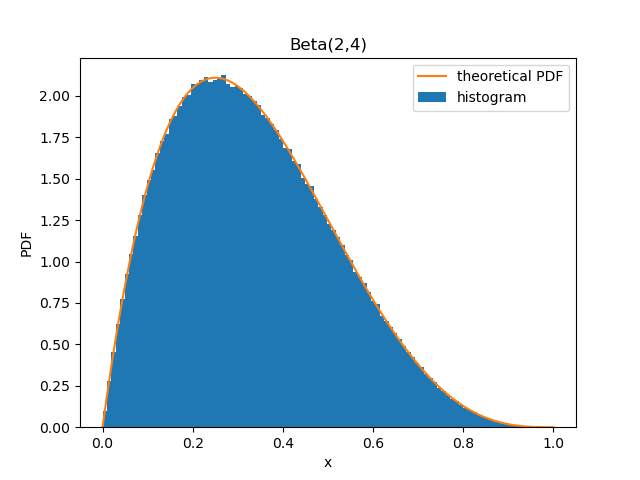
\includegraphics[width=0.9\textwidth]{../result/beta.png}
    \caption{Histogram and theoretical PDF of $Beta(2,4)$}
\end{figure}

(b) Similarly with (a), we want to sample on $N(0,1)$ with acceptance-rejection algorithm.\\
Let $Z\sim N(0,1)$, and $X=|Z|$.\\
So $Z\in (-\infty,+\infty)$, $X\in (0,+\infty)$.\\
We can calculate the PDF of $X$:\\
$f(x)=f_X(x)=\dfrac{2}{\sqrt{2\pi}}e^{-\frac{1}{2}x^2},x>0$.\\    

And we can choose that $Y\sim Expo(1)$, and its PDF is $g(y)=f_Y(y)=e^{-y},y>0$.\\
Following the method in (a), we can get that $c\geq sup_y\dfrac{f(y)}{g(y)}$.\\
$\dfrac{f(y)}{g(y)}=\dfrac{\frac{2}{\sqrt{2\pi}}e^{-\frac{1}{2}y^2}}{e^{-y}}=\dfrac{2}{\sqrt{2\pi}}e^{-\frac{1}{2}y^2+y}$.\\
Since $y>0$, so we can get that when $y=1$, $\dfrac{f(y)}{g(y)}$ will take the maximum value within the domain.\\
i.e. $sup_y\dfrac{f(y)}{g(y)}=\dfrac{f(1)}{g(1)}=\dfrac{2}{\sqrt{2\pi}}e^{-\frac{1}{2}+1}=\sqrt{\dfrac{2e}{\pi}}$.\\
So we can just take $c=\sqrt{\dfrac{2e}{\pi}}$.\\

Then we can do the acceptance-rejection algorithm.\\
1. Generate $Y\sim Expo(1)$.\\
2. Generate $U\sim Unif(0,1)$.\\
3. If $U\leq \dfrac{f(Y)}{c\cdot g(Y)}=\dfrac{\frac{2}{\sqrt{2\pi}}e^{-\frac{1}{2}Y^2}}{\sqrt{\frac{2e}{\pi}}\cdot e^{-Y}}=\dfrac{1}{\sqrt{e}}e^{-\frac{1}{2}Y^2+Y}=e^{-\frac{1}{2}(Y-1)^2}$, then set $X=Y$\\
4. Else, go back to step 1.\\

After that, we can get the sample the distribution of $X$.\\
To sample on $Z\sim N(0,1)$, since $X=|Z|$, so we can generate $U'\sim Unif(0,1)$,\\
and let $Z=\begin{cases}
    X, & U'\leq \frac{1}{2}\\
    -X, & U'>\frac{1}{2}
\end{cases}$.\\
After that, we can sample the distribution of $Z\sim N(0,1)$ with acceptance-rejection method.\\

\begin{figure}[H]
    \centering
    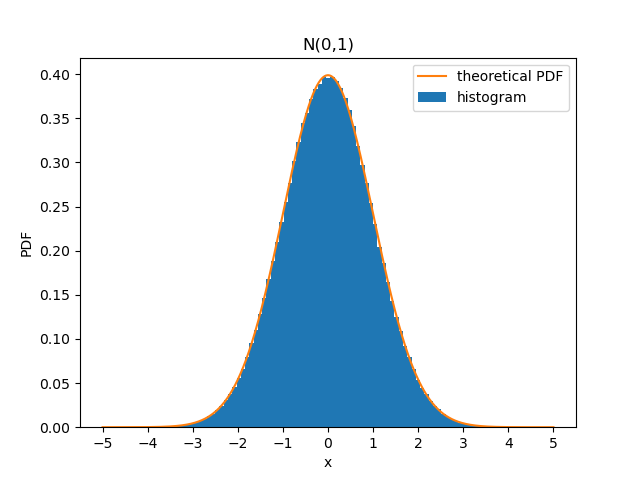
\includegraphics[width=0.9\textwidth]{../result/normal.png}
    \caption{Histogram and theoretical PDF of $N(0,1)$}
\end{figure}

Prove the correctness of the algorithm in theorem:\\
1. Let event $A = "U \leq \dfrac{f(Y)}{c\cdot g(Y)}"$.\\
From the decription of the algorithm, we know that we let $X=Y$ when $A$ happens.\\
So the PDF of generated r.v.s. $X$ is that $f_Y(y|A)=\dfrac{P(A|Y=y)}{P(A)}\cdot f_Y(y)$.\\

2. And $P(A|Y=y)=P(U\leq \dfrac{f(Y)}{c\cdot g(Y)}|Y=y)=P(U\dfrac{f(y)}{c\cdot g(y)}|Y=y)$.\\
Since $U$ and $Y$ are independent, so $P(U\leq \dfrac{f(y)}{c\cdot g(y)}|Y=y)=P(U\leq \dfrac{f(y)}{c\cdot g(y)})$.\\
And since $U\sim Unif(0,1)$, so $P(U\leq \dfrac{f(y)}{c\cdot g(y)})=\dfrac{f(y)}{c\cdot g(y)}$.\\
So $P(A|Y=y)=\dfrac{f(y)}{c\cdot g(y)}$.\\

3. As for $P(A)$, with LOTP, we can get that\\
$P(A)=\int_{0}^{+\infty}P(A|Y=y)g(y)dy$.\\
From 2., we get that $P(A|Y=y)=\dfrac{f(y)}{c\cdot g(y)}$.\\
So $P(A)=\int_{0}^{+\infty}\dfrac{f(y)}{c\cdot g(y)}g(y)dy=\dfrac{1}{c}\int_{0}^{+\infty}f(y)dy=\dfrac{1}{c}$.\\
For the last step, this is because $g(y)$ is the PDF of $Expo(1)$, which support is $(0,+\infty)$, so $\int_{0}^{+\infty}g(y)dy=1$.\\

4. Combine 2., 3. into 1., we can get that\\
$P(Y=y|A)=\dfrac{P(A|Y=y)}{P(A)}\cdot f_Y(y)=\dfrac{\frac{f(y)}{c\cdot g(y)}}{\frac{1}{c}}\cdot g(y)=f(y)$.\\

So from 1. to 4., we have prove that the PDF of generated r.v.s. $X$ is that $f_Y(y|A)=f(y)$.\\
i.e. $X\sim f(y)$.\\

And since $X=|Z|$, so we generated a r.v.s. $U'\sim (0,1)$.\\
And let $Z=\begin{cases}
    X, & U'\leq \frac{1}{2}\\
    -X, & U'>\frac{1}{2}
\end{cases}$.\\

This is because $Z\sim(0,1)$, so it is symmetric about $x=0$.\\
And since $X=|Z|$, so it can be regard that $X$ takes the value of $Z$ with probability $\frac{1}{2}$, and takes the value of $-Z$ with probability $\frac{1}{2}$.\\
So we can generate $X$ with $U'\sim (0,1)$, and let $X=Z$ when $U'\leq \frac{1}{2}$, and let $X=-Z$ when $U'>\frac{1}{2}$.\\

So above all, we can generate $Z\sim N(0,1)$ with acceptance-rejection method. The correctness have been proved.\\

(c) Both Acceptance-Rejection method and Box-Muller method can be used to sample on $N(0,1)$. And each of them have their own pros and cons\\
As for the Acceptance-Rejection method:
\begin{itemize}
    \item Pros:
    \begin{itemize}
        \item 1. It is easy to implement.
        \item 2. It can be used to sample on any distribution, we do not have to need the exact expression of the distribution that we want to sample,
                 we only need to know the relativeness.
        \item 3. It can sample on any distribution, not only $N(0,1)$.
    \end{itemize}
    \item Cons:
    \begin{itemize}
        \item 1. It may be difficult to find a suitable constant $c$.
        \item 2. It may be slower to sample because for each time, the probability of acceptance $\sim FS(p)$, where $p=\dfrac{1}{c}$, so the expected sample time is $\dfrac{1}{p}=\dfrac{1}{\frac{1}{c}}=c$.
                 So it may takes $c$ times to get one sample compared with Box-Muller method.
        \item 3. The quantity of the sample points is not fixed, it depends on the constant $c$. If $c$ is too big, then it may takes a lot of time to get one sample, and if it is too small, it may loss the accuracy.
    \end{itemize}
\end{itemize}
As for the Box-Muller method:
\begin{itemize}
    \item Pros:
    \item \begin{itemize}
        \item 1. It is easy to implement.
        \item 2. It is fast.
        \item 3. It is accurate.
        \item 4. It is easy to generate two independent $N(0,1)$ r.v.s.
    \end{itemize}
    \item Cons:\\
    \begin{itemize}
        \item 1. It can only be used to sample on $N(0,1)$.
        \item 2. It requires the exact expression of the distribution that we want to sample.
        \item 3. It requires the trigonometric function and exponential functon, which is advanced, and may be difficult to implement.
    \end{itemize}
\end{itemize}
So above all, Acceptance-Rejection method can be used to sample on various distributions, but it may be slow and difficult to find a suitable constant $c$.\\
Box-Muller method can only be used to sample on $N(0,1)$, but it is fast and accurate.\\

(d) To calculate $c=P(Y>8)$, where $Y\sim N(0,1)$.\\
So the PDF of $Y$ is that $f(y)=\dfrac{1}{\sqrt{2\pi}}e^{-\frac{1}{2}y^2}$.\\
It may be difficult to calculate the exact value of $c$ using simple sampling methods (because of the 3$\sigma$'s principle, the result must be very small).\\
So we can use the importance sampling.\\
Take $g\sim N(8,1)$.\\
Let $Y_1,\cdots,Y_N\sim g$, so the PDF of $g$ is that $g(y_j)=\dfrac{1}{\sqrt{2\pi}}e^{-\frac{1}{2}(y_j-8)^2}$.\\
Let $h(Y_j)$ be the indicator that whether $Y_j>8$.\\

So with monty carlo method, we can get that\\
$c=P(Y>8)=E[I(Y>8)]=\dfrac{1}{n}\sum_{j=1}^nI(Y_j'>8)=\dfrac{1}{n}\sum_{j=1}^nh(Y_j')$,
where $Y_j'\sim N(0,1)$.\\

With importance sampling, since $I=E_f[h(Y)]=\int h(y)f(y)dy=\int\dfrac{h(y)f(y)}{g(y)}g(y)dy=E_g[\dfrac{h(Y)f(Y)}{g(Y)}]$.\\
So $I'=\dfrac{1}{n}\sum\limits_{i=1}^n\dfrac{h(Y_j)f(Y_j)}{g(Y_j)}$, where $Y_j\sim N(8,1)$.\\
we can get that $c'=\dfrac{1}{n}\sum_{j=1}^n\dfrac{h(Y_j)f(Y_j)}{g(Y_j)}$\\
$=\dfrac{1}{n}\sum_{j=1}^nI(Y_j>8)\cdot \dfrac{\frac{1}{\sqrt{2\pi}}e^{-\frac{1}{2}Y_j^2}}{\frac{1}{\sqrt{2\pi}}e^{-\frac{1}{2}(Y_j-8)^2}}$\\
$=\dfrac{1}{n}\sum_{j=1}^nI(Y_j>8)\cdot e^{-8Y_j+32}$\\

So we just need to sample $n$ times, $Y_j\sim N(0,8)$, and calculate the average of $I(Y_j>8)\cdot e^{-8Y_j+32}$.\\

\begin{figure}[H]
    \centering
    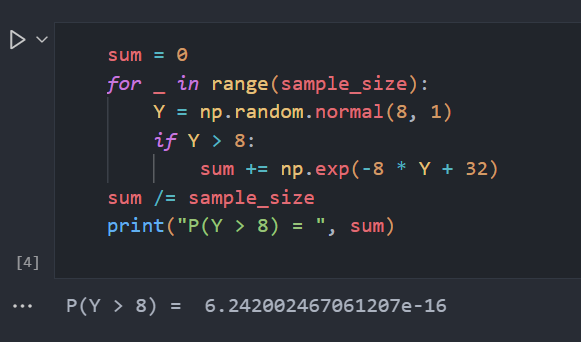
\includegraphics[width=0.9\textwidth]{../result/importance.png}
    \caption{$P(Y>8),\ Y\sim N(0,1)$}
\end{figure}

The result using important sampling method is $6.242002467061207e-16$.\\
Which is very close to the correct answer $6.25*10^{-16}$.\\
So we can regard that the importance sampling method is effective and provide correct answers.\\

The following are the pages from jupyter notebook to show that the code can successful run out the images and calculation results we mentioned above.\\

\end{homeworkProblem}

\newpage

\end{document}
